% !TEX program = xelatex
\documentclass[UTF8,fontset=windows,oneside]{ctexbook}

\usepackage{amsmath}
\usepackage{amssymb}
\usepackage{extarrows}
\usepackage{graphicx}
\usepackage{color}

\begin{document}
\section*{第一周}
\subsection*{1.1 运动积分与运动方程}
已知带电荷$e$的质量为$m$的粒子在沿$z$轴方向磁感应强度为$B$的磁场运动时的拉格朗日量为:
\[L=\frac{1}{2}m\left(\dot{x}^2+\dot{y}^2+\dot{z}^2\right)+\frac{eB}{2}(x\dot{y}-y\dot{x})\]
(a) 求出正则动量$p_x,p_y,p_z$,并且根据循环坐标指出哪个是守恒量?\\
(b) 求出系统的哈密顿量并写下正则方程(不需要求解).\\
(c) 根据正则方程,写下对应的两个守恒量(运动积分).\\
(d) 其实也不用这么复杂,根据拉格朗日量写下运动方程(不要求解),重新得出前面你得到的三个守恒量.\\
(e) 对于本题,高中时就已然知晓粒子的运动,在不解运动方程的情况下直接解释$x p_y-y p_x$的物理含义并由此说明它是一个守恒量.\\
*(f) 其实前面得到的四个守恒量都可以根据对称性得到,阅读下面相关材料并继续作答:

{
    \itshape
    Noether定理指出每个连续对称性都对应一个守恒量. 所谓连续对称性就要涉及无穷小的对称操作,考虑对广义坐标的无穷小变换:$\mathbf{q}\rightarrow\mathbf{q}+\delta\mathbf{q}$. 其中
    无穷小量$\delta\mathbf{q}$的具体形式由对称操作本身决定. 比如对于平移对称性,$\delta q=\epsilon$是一个无穷小常数;对于旋转不变性(考虑直角坐标情形),$\delta \mathbf{r}=\delta\mathbf{\phi}\times\mathbf{r}$,
    其中$\delta\mathbf{\phi}$是一个无穷小转角,方向沿转轴方向,由右手螺旋定则确定.

    我们便能写出在这一对称操作下拉格朗日量的变化(保留到一阶$\mathcal{O}(\delta\mathbf{q})$)$\delta L$,如果$\delta L=0$,也就是说在这个对称操作下拉格朗日量不变,
    那自然作用量$S$也就不变,由变分法导出的运动方程也就没变,而一个系统最重要的就是运动方程,也就是说在这个操作下系统没有发生变化,所以才叫做\textbf{对称操作}.
    不过$\delta L=0$这个条件还是太苛刻了,即使我们最初接触到Noether定理的时候空间平移对称性和空间各向同性以及时间平移对称性确实有$\delta L=0$,不过我们完全
    可以把条件放宽一些,因为拉格朗日量有一个最重要的性质就是\textbf{规范不变性:拉格朗日量之间可以相差一个任意函数的关于时间的全导数}.也就是说$\delta L=-\frac{dG}{dt}$时\footnote{这里的负号是为了后面结论的美观},操作实际上也是对称操作,
    不会改变系统运动方程. 我们作如下推演\footnote{对于多维情况,省略了求和符号和下标,请自行脑补}:
    \begin{align*}
        \delta L&=L(q+\delta q,\dot q+\delta \dot q,t)-L(q,\dot q,t)\\
        &=\frac{\partial L}{\partial q}\delta q+\frac{\partial L}{\partial \dot q}\delta \dot q + \mathcal{O}(\delta q)\\
        &=\frac{d}{dt}\left(\frac{\partial L}{\partial \dot q}\right)\delta q+\frac{\partial L}{\partial \dot q}\delta\dot q+ \mathcal{O}(\delta q)\\
        &=\frac{d}{dt}\left(\frac{\partial L}{\partial \dot q}\delta q\right)+ \mathcal{O}(\delta q)
    \end{align*}
    略去高阶小量并根据$\delta L=-\frac{dG}{dt}$,我们得到:
    \begin{equation}
        \boxed{
            \frac{d}{dt}\underbrace{\left(\frac{\partial L}{\partial \dot q}\delta q+G\right)}_{\equiv J}=0
        }
    \end{equation}
    我们便完全根据对称性导出了一个守恒量$J$!\footnote{这个定理还有许多证明方式(我至少还看到过两种),这里列出的是经典力学中很容易理解的证明.}
}\\
\textbf{Question1}:分别根据$x,y,z$方向的平移对称性导出你在$(a)\sim(d)$中导出的三个守恒量.\\
\textbf{Question2}:根据系统关于$z$轴方向上的旋转对称性导出$(e)$中的守恒量.

\subsection*{1.2 中心势场散射}
\noindent(a) 考虑一个能量为$E$的粒子从势能为$0$的上半平面入射到势能为$-V_1$(吸引势)的下半平面。试证明粒子的折射规律类似于光的折射定律,满足:
\[\sin \theta_0=n\sin \theta_1\quad(n=\sqrt{1+V_1/E})\]
其中$\theta_0$和$\theta_1$分别为入射角和折射角.\\
(b) 对于下面的球形吸引势场,求出对应的微分散射截面:
\begin{equation*}
    V(r)=
    \begin{cases}
        -V_1 & r\leq a\\
        0 &r>a
    \end{cases}
\end{equation*}

\textbf{注}:{\itshape 对于任意一个势场,其实我们都可以通过积分计算轨道从而计算偏转角得到微分散射界面,但是操作性不强,所以一般来说让我们实际去求的要么是可以直接从几何上得到偏转角,
要么是特殊形式的势场,容易直接积分.}

\subsection*{1.3 比较巧妙的方法计算中心势场散射}
尝试计算下面的中心势场的微分散射截面:
\begin{equation*}
    V(r)=
    \begin{cases}
        \frac{\alpha}{r}-\frac{\alpha}{R} & r\leq R\\
        0 &r>R
    \end{cases}
\end{equation*}
这道题直接用书上公式积分你是算不出来的。

\subsection*{1.4 函数的Legendre展开}
\noindent(a) 将$x^2$在$\left[-2,3\right]$上展开为Legendre多项式(提示,先将函数变换到$\left[-1,1\right]$上).\\
(b) 将 $\sqrt{1-2xt+t^2}$ 在$\left[-1,1\right]$上展开为Legendre多项式.\footnote{本题为书上P266原题}\\
可能用得到的公式:\footnote{第一个递推式建议牢记}
\begin{align*}
    &P_{l+1}^\prime(x)-P_{l-1}^\prime(x)=(2l+1)P_l(x)\\
    &P_{2n+1}(0)=0,\quad P_{2n+1}^\prime(0)=\frac{(-1)^n(2n+2)!}{2^{2n+1}n!(n+1)!}\\
    &P_{2n}(0)=(-1)^n\frac{(2n)!}{2^{2n}(n!)^2},\quad P^\prime_{2n}(0)=0
\end{align*}

\subsection*{1.5 Gamma函数与极限}
已知Stirling公式:
\begin{equation}
	\label{eq:2}
    \lim_{n\to\infty}\frac{e^nn!}{n^n\sqrt{n}}=\sqrt{2\pi}
\end{equation}
或者你也可以简单的认为是在$n$很大时:
\begin{equation}
    n!\sim\sqrt{2\pi n}\left(\frac{n}{e}\right)^n
\end{equation}
根据上面的公式,求极限(并没有要求极限过程中$n\in\mathbb{Z}$):\footnote{求解过程不必强调严谨性}
\[\lim_{n\to\infty}\frac{\Gamma(2n)}{\sqrt{n}\Gamma(2n-1/2)}\]

\section*{第二周}
\subsection*{2.1 留数定理计算积分}
计算下面的积分:
\begin{equation}
    I=\int_{0}^{\pi}\frac{\cos n\varphi}{1+2p\cos\varphi+p^2}\mathrm{d}\varphi,\quad 0<p<1,n\in \mathbb{N}
\end{equation}
{\itshape \textbf{Answer}}:$\frac{\pi(-p)^n}{1-p^2}$

\subsection*{2.2 水星近日点进动与三维各项同性谐振子}
\noindent $(a)$在极坐标下根据能量守恒和角动量守恒导出下面的在中心势场$V(r)$作用下的积分形式的轨道方程:
\begin{equation}
    \theta-\theta_0=\int_{r_0}^{r}\frac{dr}{r^2\sqrt{\frac{2m}{J^2}(E-V)-\frac{1}{r^2}}}\xlongequal{u=\frac{1}{r}}-\int_{u_0}^{u}\frac{du}{\sqrt{\frac{2m}{J^2}(E-V)-u^2}}
\end{equation}
其中$E$是总能量,$J$是轨道角动量。\\
$(b)$众所周知中心势场下只有两类轨道是闭合的,一类是反比势场,一般的运动轨迹是圆锥曲线;另一类是胡克势,$V(x)=\frac{1}{2}m\omega^2r^2$,回答下列问题:\\
\textbf{Question1}:根据(a)中得到的积分形式轨道方程得到胡克势下的运动轨道方程:
\begin{equation}
    \frac{J^2}{mE}\frac{1}{r^2}=1+\sqrt{1-\frac{\omega^2J^2}{E^2}}\cos 2(\theta-\theta_0)
\end{equation}
\textbf{Question2}:说明上面得到的轨道实际上是以力心为几何中心的椭圆轨道,且证明:
\[E=\frac{1}{2}m\omega^2(a^2+b^2),\quad J=m\omega ab\]
其中$a$和$b$分别为椭圆的长半轴和短半轴。\\
\textbf{Question3}:从“面积速度”这一概念出发推导轨道周期和$\omega$的关系,在解答$(a)$时,一个副产物是$r(t)$的积分表达式,现在根据它推导:
\begin{equation}
    r^2(t)=\frac{E}{m\omega^2}\left[1-\sqrt{1-\frac{\omega^2J^2}{E^2}\cos 2\omega(t-t_0)}\right]
\end{equation}

\noindent $(c)$如果势能稍稍偏离$\frac{k}{r}$,比如因为有其它行星的吸引,这时轨道不再是闭合的椭圆轨道,由于$\delta V(r)$很小,所以可以预料到新的轨道是在原先的椭圆轨道基础上加上一个进动,如下图(\ref{fig:1})所示:
\begin{figure}[h]
    \centering
    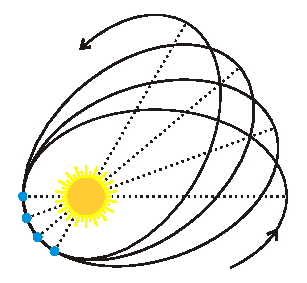
\includegraphics[scale=0.8]{水星进动.pdf}
    \caption{水星轨道进动示意图}
    \label{fig:1}
\end{figure}

\noindent 现在请根据$(a)$,推导对于一般的微扰$\delta V(r)$,轨道每周期的近日点进动量:
\begin{equation}
    \Delta \theta = 4mJ\frac{\partial}{\partial(J^2)}\int_{r_{\min}}^{r{\max}}\frac{\delta V(r)}{\sqrt{2m(E+\frac{k}{r})-\frac{J^2}{r^2}}}\mathrm{~d}r
\end{equation}
\textbf{提示}:{\itshape 对于$\frac{k}{r}$势,式(5)在一个周期内的积分是$2\pi$,也即一周期后行星完全回到原先的位置。但现在有微扰,所以运行一周后$\theta-\theta_0\neq 2\pi$,会和原先的位置有个偏差$\Delta \theta$.
你要做的就是在合适的近似下算出这个进动角,你可以放心大胆地使用费曼积分法\footnote{就是积分和求导可以互换顺序}。}\\
$(d)$ 水星近日点也存在上面的进动现象,天文观测表明大约为每世纪$5600^{\prime\prime}$,根据牛顿理论考虑天文观测的岁差以及其它星体的吸引导致的$\delta  V\neq 0$,可以解释其中的$5557^{\prime\prime}$,
还有$43^{\prime\prime}$无法用经典理论解释。这里面一部分是由于狭义相对论,一部分是由于广义相对论,狭义相对论效应的修正是非常非常小的,我们下面来具体考虑一下SR的修正。\\
\textbf{Question1}:考虑相对论效应后可以将此问题的拉式量写为:
\[\mathcal{L}=-mc^2\sqrt{1-\frac{v^2}{c^2}}+\frac{k}{r}\]
现在考虑到$v\ll c$,将$\mathcal{L}$展开到$v^4/c^4$,忽略掉静止质能项$mc^2$,与经典情况对比,得到对应的微扰项({\itshape \textbf{Answer}:$-\frac{mv^2}{8}\left(\frac{v^2}{c^2}\right)$})。\\
\textbf{Question2}:我们用$E$表示除去静止质能后的总能量,由于相对论修正实在太小,所以我们可以认为它依旧是经典情况下的$E\approx -\frac{k}{r}+\frac{1}{2}mv^2$. 现在根据此关系将$\delta V$中的$v^2$全部替换成$E$相关的式子,再根据
$(c)$中推导的公式计算每周期的近日点进动量。\footnote{由于我们只考虑一阶修正,所以积分时的上下限依旧根据经典情况,也就是$\delta V=0$,用$E,J$去确定积分上下限所满足的方程。计算时别忘了$u=1/r$换元。}\\
{\itshape\textbf{Answer:}}
\[
   \quad\Delta\theta=\frac{\pi k^2}{J^2c^2}=\frac{\pi GM_\odot}{a(1-e^2)c^2}
\]
\textbf{Qurstion3}:上网查找相关数据,根据$(c)$中结果求出每世纪由于狭义相对论导致的水星近日点进动修正量.\\
\textbf{积分表}:
\begin{equation*}
    \int{\frac{dx}{\sqrt{a^2-x^2}}}\xlongequal{\text{令}x=a\cos\theta}-\arccos\left(\frac{x}{a}\right)
\end{equation*}
\begin{align*}
    \int \frac{{{{(ax + b)}^2}}}{{{x^2}\sqrt {(ax + b) - {c^2}} }}dx=&- \frac{{b\sqrt {(ax + b) - {c^2}} }}{x}\\
    &- \frac{{{a^2}}}{c}\operatorname{arccot} \left( {\frac{{2c\sqrt {(ax + b) - {c^2}} }}{{a - 2{c^2}x}}} \right)\\
    &- \frac{3}{2}a\sqrt b \operatorname{arctanh} \left( {\frac{{ax + 2b}}{{2\sqrt b \sqrt {(ax + b) - {c^2}} }}} \right)
\end{align*}
\textbf{Qurstion3}:广义相对论带来的修正实际上可以用一个与距离的立方成反比的微扰势来描述,也即:
\[\delta V=\frac{kJ^2}{m^2c^2},k\equiv GM_\odot m\]
试用上面的进动角计算公式计算广义相对论预言的水星近日点进动修正量。\\
{\itshape\textbf{Answer:}}
\[\bar{\dot{\theta}}=\frac{6\pi}{(1-e^2)T}\left(\frac{R_S}{a}\right)\approx 42.98^{\prime\prime}\text{per century},R_s\equiv GM_\odot/c^2\]
\subsection*{2.3 柱内球}
半径为$a$,质量为$m$的匀质球在半径为$b(b>a)$的无限高内面粗糙固定圆柱的内壁上作纯滚动。试证明其质心在铅直方向上作简谐运动。
\begin{figure}[h]
    \centering
    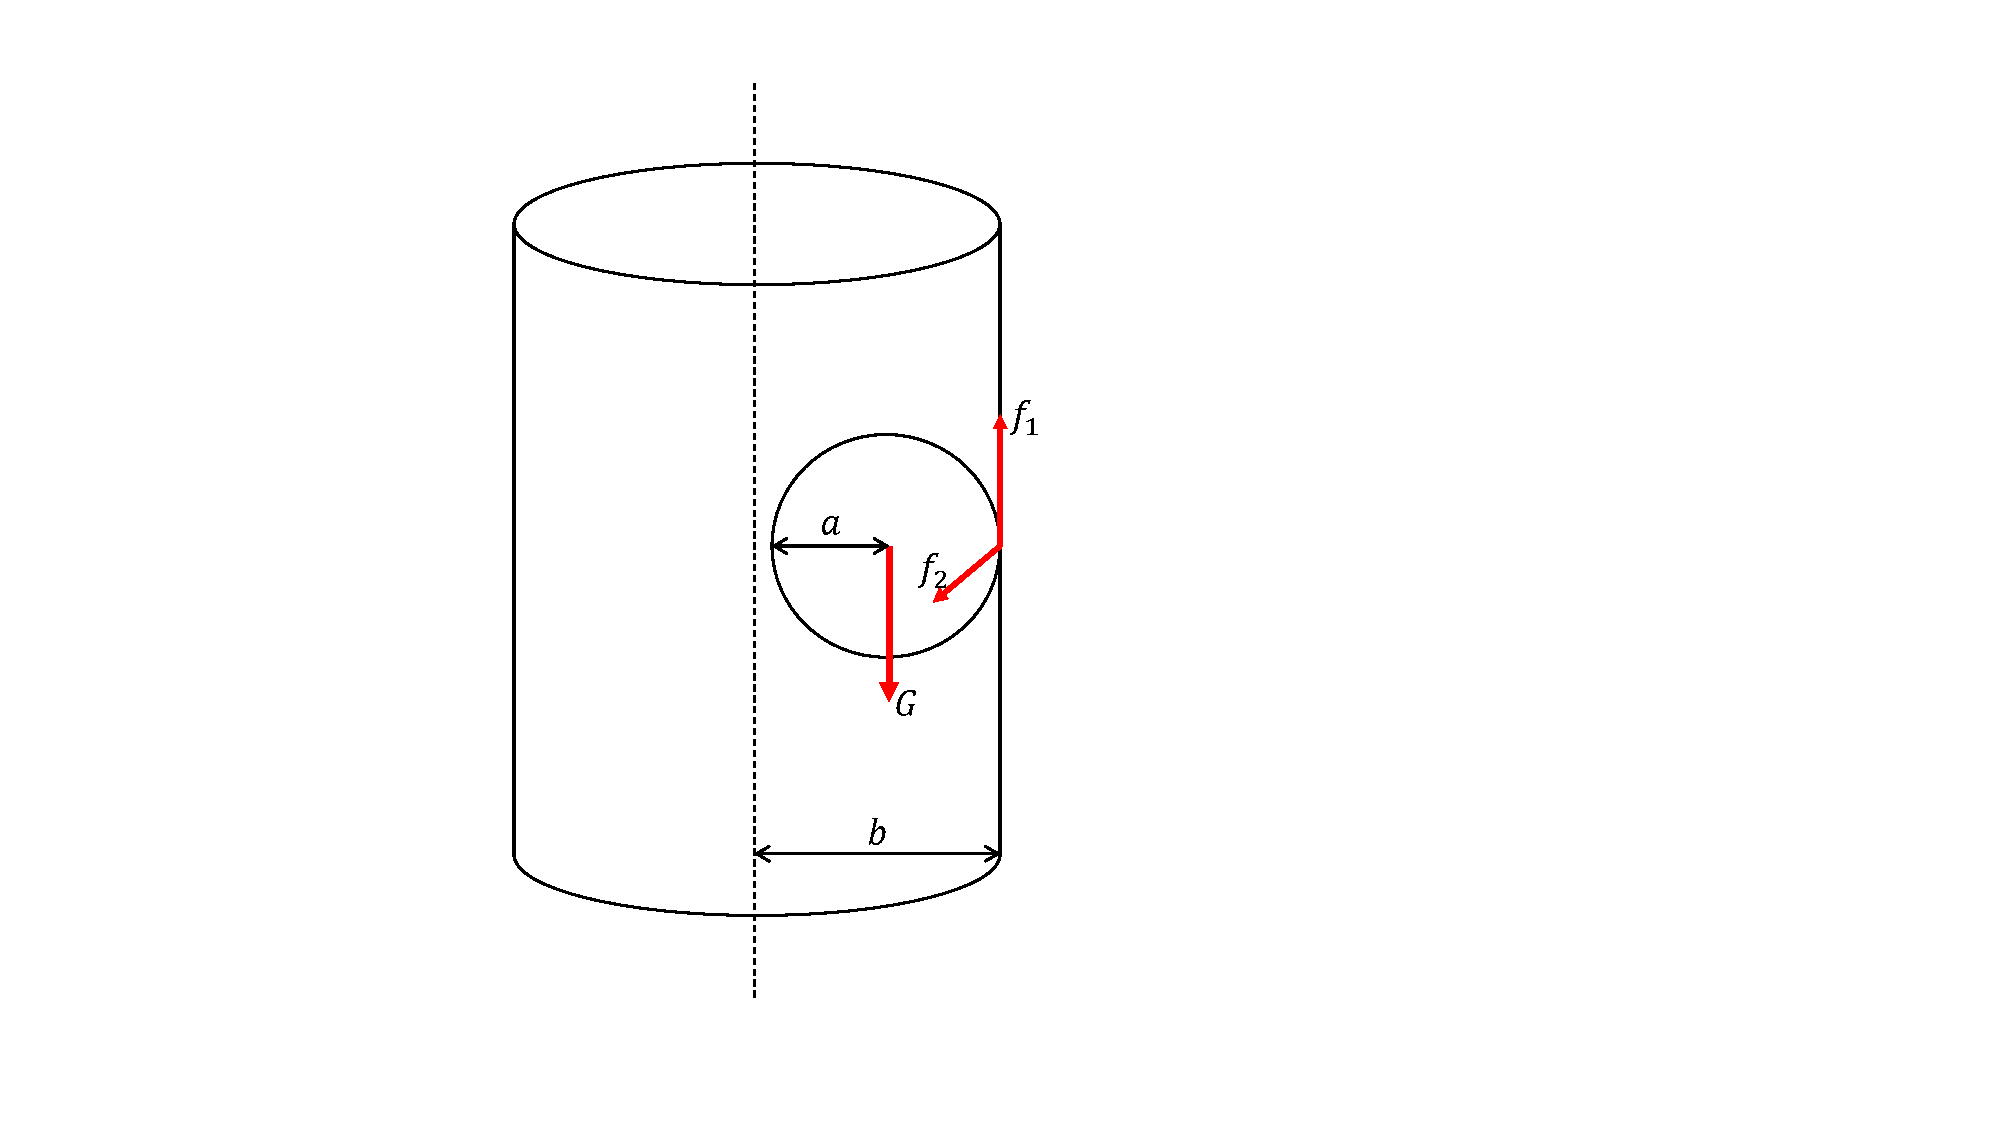
\includegraphics[scale=0.4]{2-3.pdf}
    \caption{题2.3图}
    \label{fig:2}
\end{figure}

\noindent{\itshape\textbf{Hint}:这个题难点之一在坐标系的选取,讨论这个问题首先肯定要取一个质心系,然后根据受力情况,最简单的选择是选取一个转动系,某一个轴始终和接触点固连,
但是这样选取的动系并不是与球固连的,会导致在列Euler动力学方程时有新的麻烦。这个系下列出的运动方程最简单,但是需要你深刻理解Euler方程。当然你也可以选别的参考系,计算量更大。}

\section*{第三周}
\subsection*{3.1 Poisson括号}
\subsubsection{\uppercase\expandafter{\romannumeral 1}.Poisson判据}
\begin{itemize}
	\item[$(a)$] 证明$\frac{df}{dt}=[f,H]+\frac{\partial f}{\partial t}$.
	\item[$(b)$] 证明Poisson定理:如果任意的两个力学量$f,g$({\color{red}并不要求它们不显含时间})是运动积分,那么$[f,g]$也是.
	\item[$(c)$] $\mathbf{L}\equiv \mathbf{r}\times\mathbf{p}$,证明其分量满足$[L_i,L_j]=\epsilon_{ijk}L_k$. 阐述你从中发现了什么有趣的定理.\footnote{不要问算这个泊松括号的时候是如何选取正则坐标的,泊松括号是正则不变量,你要不信就试着证明它.}
\end{itemize}
\subsubsection{\uppercase\expandafter{\romannumeral 2}.Lagrange括号}
既然前面是把$f,g$看作是$2n$个正则坐标的函数,那么反过来也可以把$q,p$看作是$2n$个独立的力学量的函数,从而定义Lagrange括号:\footnote{下面的练习仅仅作微积分联系,因为这玩意没太大用其实,已经被抛弃了}
\begin{equation}
	\{\mathbf{f},\mathbf{g}\}\equiv \frac{q_i}{f}\frac{p_i}{g}-\frac{p_i}{f}\frac{q_i}{g}
\end{equation}
试证明:
\begin{equation}
	\{\mathbf{u},\mathbf{u}\}[\mathbf{u},\mathbf{u}]=-\mathbf{1}
\end{equation}
其中$\{\mathbf{u},\mathbf{u}\}$是一个$2n\times 2n$的矩阵第$i$行第$j$列是$\{\mathbf{u}_i,\mathbf{u}_j\}$,$[\mathbf{u},\mathbf{u}]$定义类似.

\subsubsection{\uppercase\expandafter{\romannumeral 3}. LRL矢量与三维谐振子守恒张量}
\begin{itemize}
	\item[$(a)$] 对于$\frac{1}{r}$势,Laplace-Runge-Lentz矢量是一个守恒量\[\mathbf{A}=\mathbf{p}\times\mathbf{L}-\frac{\mathbf{r}}{r}\]
	\begin{itemize}
		\item[\textbf{Question1}]:证明$[r_i,L_j]=\epsilon_{ijk}r_k,[p_i,L_j]=\epsilon_{ijk}p_k,[L_i,L^2]=0,[L_i,A_j]=\epsilon_{ijk}A_k$
		\item[\textbf{Question2}]:有心力场Hamiltonian是$H=p^2/2m-1/r$,利用Poisson括号证明它的确是个守恒量.
		\item[\textbf{Question3}]*:证明$$[A_1,A_2]=-\left(p^2-\frac{2}{r}\right)L_3$$
	\end{itemize}
	\item[$(b)$]对于三维各向同性谐振子:$H=\mathbf{p}^2/2m+\frac{1}{2}m\omega^2\mathbf{r}^2$.利用Possion括号证明下面的二阶张量是守恒量:
	\begin{equation}
		A_{ij}\equiv \frac{1}{2m}\left(p_ip_j+m^2\omega^2r_ir_j\right)
	\end{equation}
	$\operatorname{Tr}A$的意义是什么?如果对自己计算水平有信心可以计算一下它的行列式$|A|=L^2\omega^2/4$
\end{itemize}
\subsection*{3.2 留数定理计算积分}
\begin{equation}
	I=\int_{-\infty}^{+\infty}\frac{\cos(2m\pi x)}{x^2+x+1}\mathrm{~d}x\quad (m>0)
\end{equation}
{\itshape\textbf{Answer}}\footnote{要注意本题是$f(x)\cos x$型的积分,先计算$f(z)e^{iz}$再取实部,直接计算$f(z)$积分会导致错误.}:$\frac{2\pi(-1)^m}{\sqrt{3}}e^{-\sqrt{3}m\pi}$
\subsection*{3.3 不用积分的积分(Laplace方法)}
\textbf{Laplace Method}: 如果$f(x)$是一个在区间$[a,b]$上二阶连续可导的函数,并且存在唯一的$x_0\in(a,b)$使得
\[f(x_0)=\min\limits_{x_0\in(a,b)}f(x)\quad \text{and}\quad f^{\prime\prime}(x_0)>0\]
那么我们有如下的极限:
\begin{equation}
	\lim_{n\to\infty}\frac{\int_{a}^{b}\mathrm{~d}x\exp[-nf(x)]}{\exp[-nf(x_0)]\sqrt{\frac{2\pi}{nf^{\prime\prime}(x_0)}}}=1
\end{equation}
Laplace方法可以推广为:
\begin{equation}
	\int_{a}^{b}\mathrm{~d}xg(x)\exp[-nf(x)]\approx g(x_0)\exp[-nf(x_0)]\sqrt{\frac{2\pi}{nf^{\prime\prime}(x_0)}}
\end{equation}
\textbf{Question1}:在$N$非常大时计算下面的积分(变化成能用Laplace方法求解的形式即可)
\begin{equation}
	Z(N,T)=2\int_{0}^{+\infty}r\mathrm{~d}re^{-\beta r^2}\left\{2\cosh\left[\frac{1}{2}\beta\epsilon\left(1+\frac{4\lambda^2r^2}{\epsilon^2N}\right)^{1/2}\right]\right\}^N
\end{equation}
\textbf{Question2}:$N!=\Gamma(N+1)$由此利用Laplace方法推导出Stirling公式.

\end{document}

